\documentclass[a4paper,11pt]{article}
\usepackage[utf8]{inputenc}
\usepackage{amsfonts}
\usepackage{amsmath}
\usepackage{amssymb}
\usepackage{xcolor}
\usepackage{graphicx}
\usepackage[polish]{babel}
\usepackage[T1]{fontenc}
\usepackage{float}
\def\\{\hfill\break}


%----------------------
\title{Projekt Egzaminacyjny}
\author{Karol Krawczykiewicz, Piotr Maszczak}
\date{Listopad 2022 -- Styczeń 2023}



\begin{document}

\maketitle
\newpage
\tableofcontents
\newpage
\section{Wstęp}

Następująca analiza dotyczy dwóch spółek działających na rynku gier wideo.


\\
CD Projekt SA (CDR) to grupa działająca w dynamicznie rozwijającej się branży elektronicznej rozrywki. Z silnym naciskiem na produkcję gier przez swoje studio deweloperskie CD Project Red oraz globalną dystrybucję cyfrową za pośrednictwem platformy GOG.com, firma osiągneła duże sukcesy i jest szanowana na całym świecie.
\\\\
11 bit studios SA (11B) to wieloplatformowy deweloper gier. Firma jest aktywna na każdym etapie tworzenia gry, z znanymi tytułami takimi jak Frostpunk i This War of Mine. Oprócz produkcji gier, grupa również wydaje gry zewnętrzne i prowadzi platformę sprzedaży internetowej. 



\section {Analiza cen spółek}


\subsection{Spółka CD Projekt}




\begin{figure}[H]
    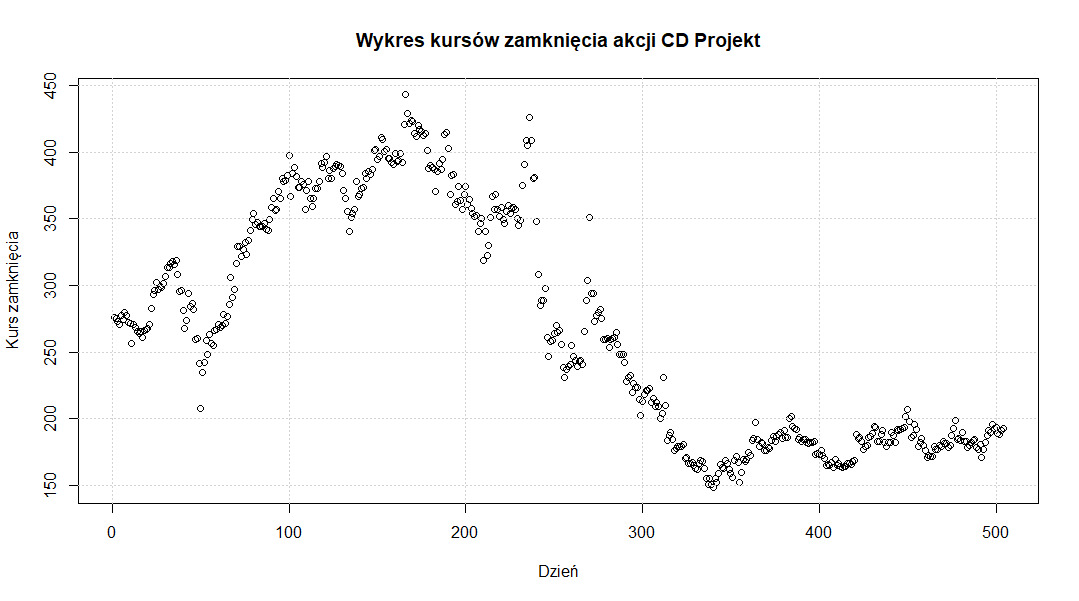
\includegraphics[width=12cm]{Wykresy CDR/CDR-kursy.png}
    \caption{Wykres akcji w przedziale czasowym od Stycznia 2020 do Grudnia 2021}
    \label{CDP-kursy}
\end{figure}
\par
\\
\par
\begin{figure}[H]
    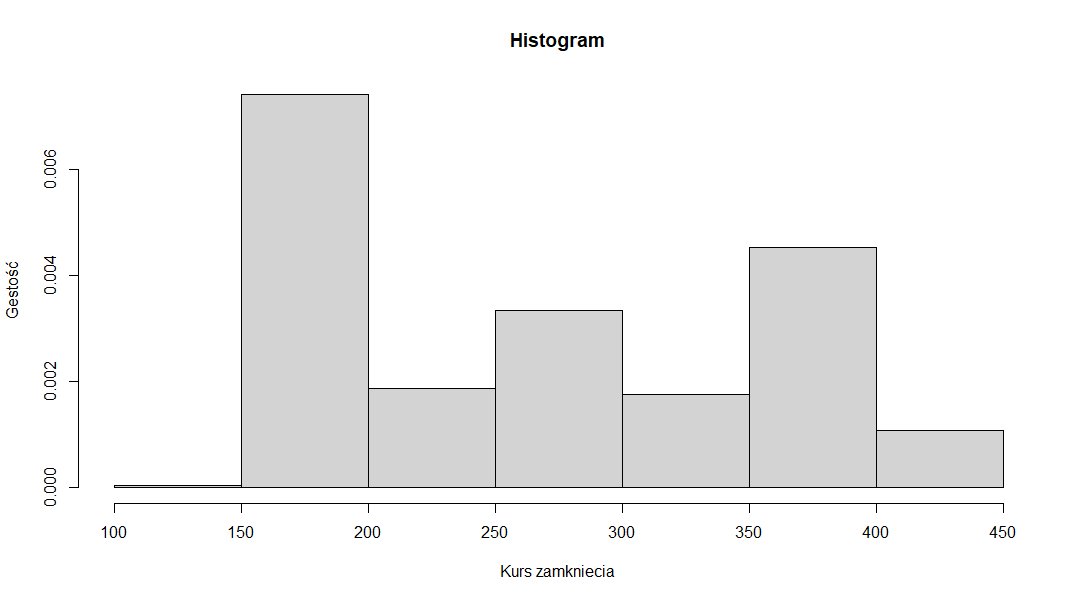
\includegraphics[width=12cm]{Wykresy CDR/CDR-histogram.png}
    \caption{Histogram gęstości}
    \label{CDP-histogram}
\end{figure}


\par
\par
\begin{table}[H]
\centering 
\begin{tabular}{|l|l|l|l|l|}
\hline
      & $\overline{x}$ & odch. st. & skośność  & kurtoza \\ \hline
Akcja & 277.6719           & 90.62922  & 0.2497853 & 1.56275 \\ \hline
\end{tabular}
\end{table}


Współczynnik skośności powyżej 0 świadczy o prawostronnej asymetrii rozkładu (wydłużone jest prawe ramię rozkładu). 
Kurtoza większa od 0 oznacza iż rozkład jest bardziej wysmukły niż normalny, większe skupienie wartości wokół średniej.

\\
\\
Wyestymowane parametry dla badanych rozkładów przy wykorzystaniu estymatora największej wiarygodności (MLE):
\begin{itemize}
  \item Rozkład normalny - mean 277.67190, sd 90.54032
  \item Rozkład log-normalny - meanlog 5.5719177, sdlog   0.3322444
  \item Rozkład gamma - shape 9.33484470 , rate  0.03362056
\end{itemize}

\begin{table}[H]
\centering 
\begin{tabular}{|l|l|l|l|l}
\cline{1-4}
                               & Normalny   & Log-normalny & Gamma      &  \\ \cline{1-4}
Kolmogorov-Smirnov statistic   & 0.1777046  & \colorbox{pink}{0.1715694}    & 0.1739537  &  \\ \cline{1-4}
Cramer-von Mises statistic     & 2.9612965  & 2.9246380    & \colorbox{pink}{2.8490879}  &  \\ \cline{1-4}
Anderson-Darling statistic     & 19.7989554 & 19.3686342   & \colorbox{pink}{19.1126404} &  \\ \cline{1-4}
Akaike's Information Criterion & 6047.228   & \colorbox{pink}{6010.751}     & 6013.699   &  \\ \cline{1-4}
Bayesian Information Criterion & 6055.697   & \colorbox{pink}{6019.220}     & 6022.168   &  \\ \cline{1-4}
\end{tabular}
\end{table}


Z powyższych danych wynika, iż rozkład Log-Normalny najlepiej opisuje kursy zamknięcia spółki CDR. Trzy z pięciu przypadków optuje za rozkładem Log-Normalny, a dwa za rozkładem Gamma. 

\begin{figure}[H]
    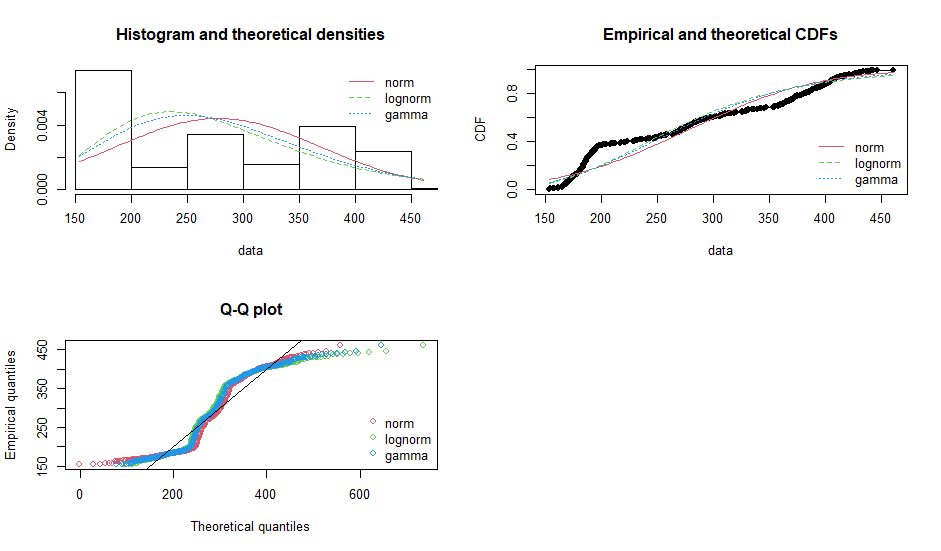
\includegraphics[width=12cm]{Wykresy CDR/CDP-estymatory.png}
    \caption{Wykresy diagnostyczne: Funkcje gęstości, Funkcja dystrybuanty, Kwantyle}
    \label{CDP-estymatory}
\end{figure}

Na podstawie wykresów diagnostycznych można wywnioskować, że prawdopodobnie żaden z rozkładów nie będzie w dobrym stopniu odwzorowywał danych.




\centerline{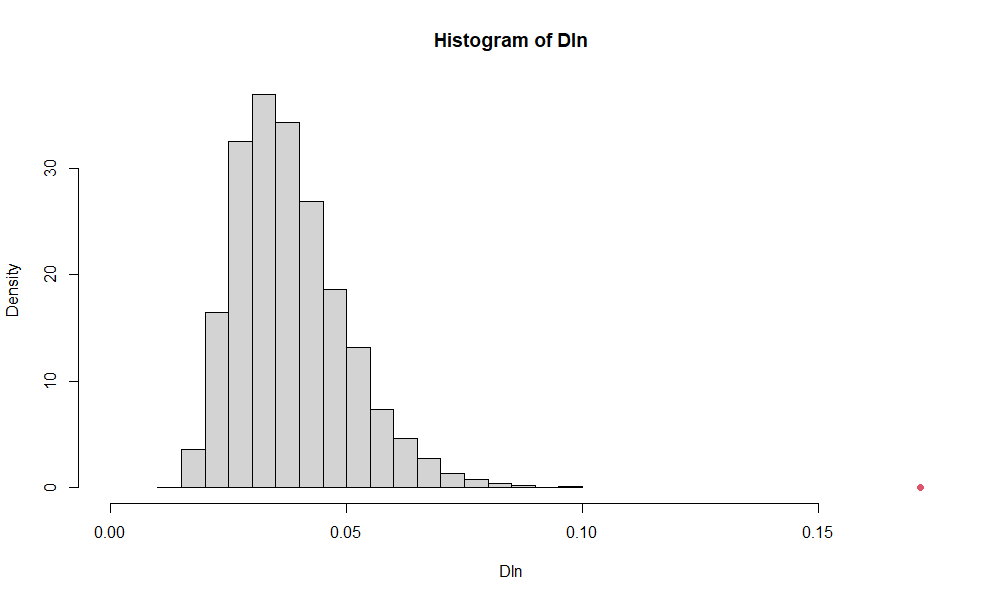
\includegraphics[width=12cm]{Wykresy CDR/CDP-MC.png}}

Po przetestowaniu hipotezy zerowej o równości dystrybuant, przy wykorzystaniu metody Monte-Carlo i statystyk Kołmogorowa-Smirnowa, uzyskano wyniki:
  $$ Dn = 0.1715694 $$
  $$p = length(Dn[Dn>dn])/N = 0$$ 
gdzie Dn to odległość dystrybuant empirycznych od rozkładu log-normalnego, dn to wartość statystyki Dn, dla danych akcji spółki, N = 10000


\\
Wartość p jest mniejsza od przyjętego poziomu istotności,

   $$ \alpha  = 5\%$$

Zatem hipotezę o równości dystrybuant odrzucamy.

%============================================================================================================
\subsection{Spółka 11 BIT STUDIOS}



\begin{figure}[H]
    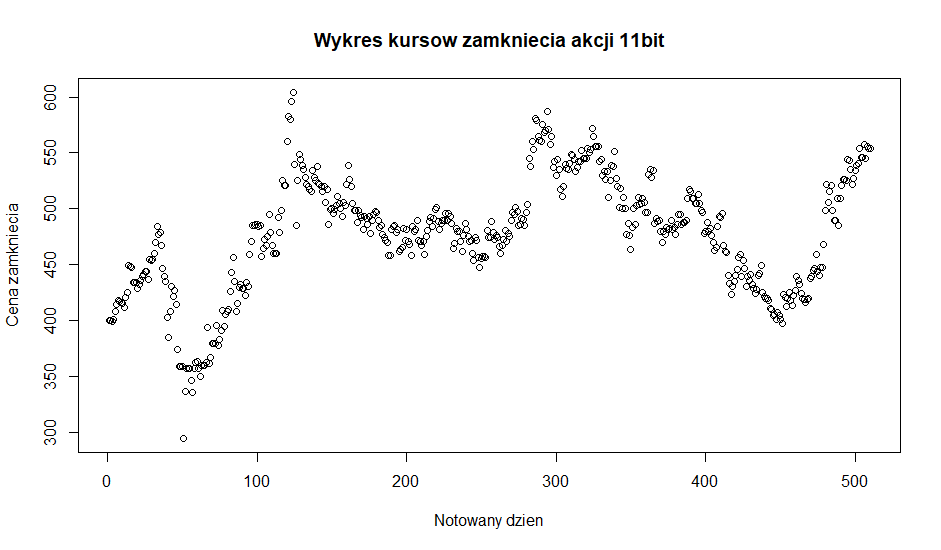
\includegraphics[width=12cm]{Wykresy 11B/11B-kursy.png}
    \caption{Wykres akcji w przedziale czasowym: Styczeń 2020 do Grudnia 2021}
    \label{11B-kursy}
\end{figure}
\par
\newpage
\par
\begin{figure}[H]
    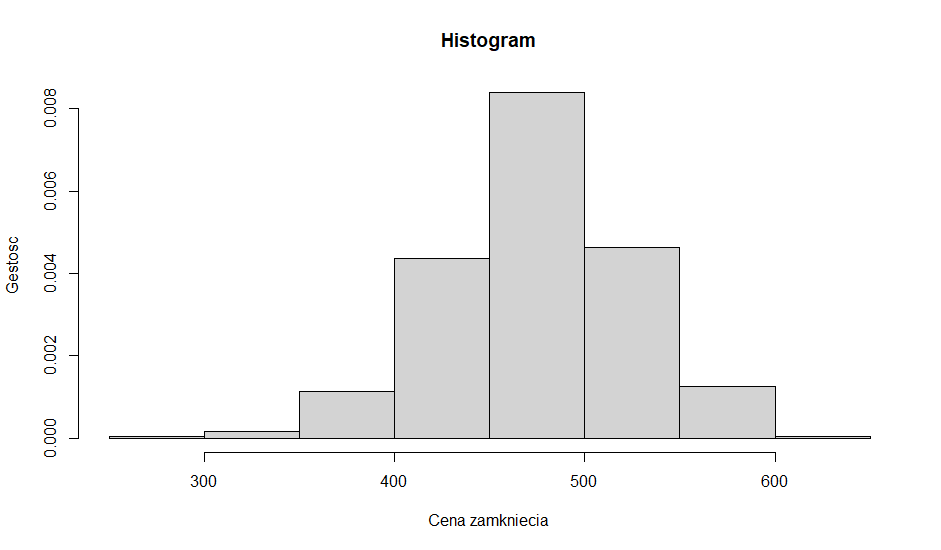
\includegraphics[width=12cm]{Wykresy 11B/11B-histogram.png}
    \caption{Histogram gęstości}
    \label{11B-histogram}
\end{figure}


\par
\par
\begin{table}[H]
\centering 
\begin{tabular}{|l|l|l|l|l|}
\hline
      & $\overline{x}$ & odch. st. & skośność  & kurtoza \\ \hline
Akcja & 476.8853     & 51.16337  & -0.385939 & 3.071287 \\ \hline
\end{tabular}
\end{table}


Współczynnik skośności poniżej 0 świadczy o lewostronnej asymetrii rozkładu (wydłużone jest lewe ramię rozkładu). Kurtoza większa od 0 oznacza iż rozkład jest bardziej wysmukły niż normalny, większe skupienie wartości wokół średniej.

\\
\\
Wyestymowane parametry dla badanych rozkładów przy wykorzystaniu estymatora największej wiarygodności (MLE):
\begin{itemize}
  \item Rozkład normalny - mean 476.88529, sd 51.11319
  \item Rozkład log-normalny - meanlog 6.1612582, sdlog 0.1111746
  \item Rozkład Weibulla -  shape 10.73364, rate 499.28283
\end{itemize}

\begin{table}[H]
\centering 
\begin{tabular}{|l|l|l|l|l}
\cline{1-4}
                               & Normalny    & Log-normalny & Weibull      &  \\ \cline{1-4}
Kolmogorov-Smirnov statistic   & 0.06995126  & 0.0929663    & \colorbox{yellow}{0.06613342}  &  \\ \cline{1-4}
Cramer-von Mises statistic     & 0.38880200  & 0.7849020    & \colorbox{yellow}{0.30039685}  &  \\ \cline{1-4}
Anderson-Darling statistic     & 2.12780717  & 4.4814222    & \colorbox{yellow}{1.55241020} &  \\ \cline{1-4}
Akaike's Information Criterion & 5464.041    & 5495.215     & \colorbox{yellow}{5455.947}   &  \\ \cline{1-4}
Bayesian Information Criterion & 5472.510    & 5503.683     & \colorbox{yellow}{5464.416}   &  \\ \cline{1-4}
\end{tabular}
\end{table}


Z powyższych danych wynika, iż rozkład Weibulla najlepiej opisuje kursy zamknięcia spółki 11 bit studios.
Wszystkie z pięciu przypadków wskazują za rozkładem Weibulla.

\begin{figure}[H]
    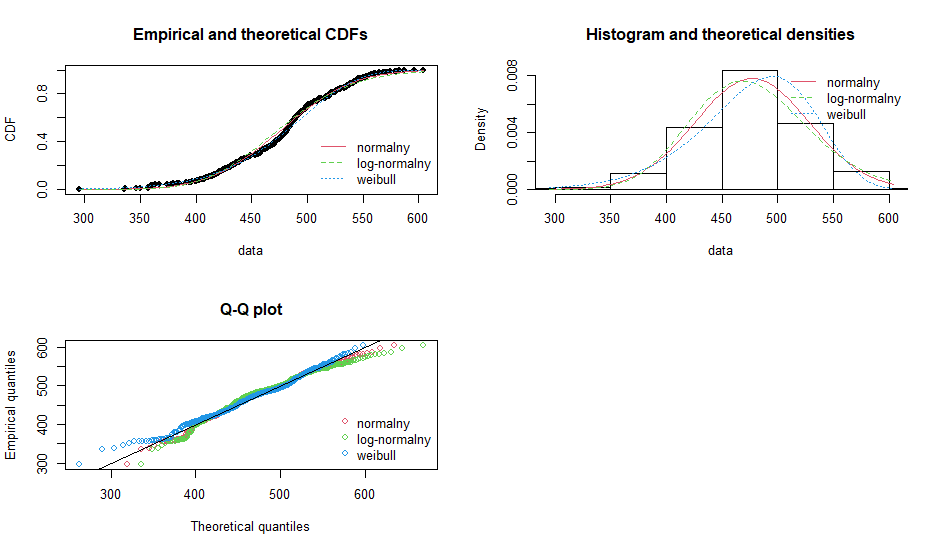
\includegraphics[width=12cm]{Wykresy 11B/11B-estymatory.png}
    \caption{Wykresy diagnostyczne: Funkcja dystrybuanty, Funkcje gęstości, Kwantyle}
    \label{11B-estymatory}
\end{figure}

Na podstawie wykresów diagnostycznych można wywnioskować, że rozkład Weibulla najbardziej odwzorowuje dane.



\newpage
\centerline{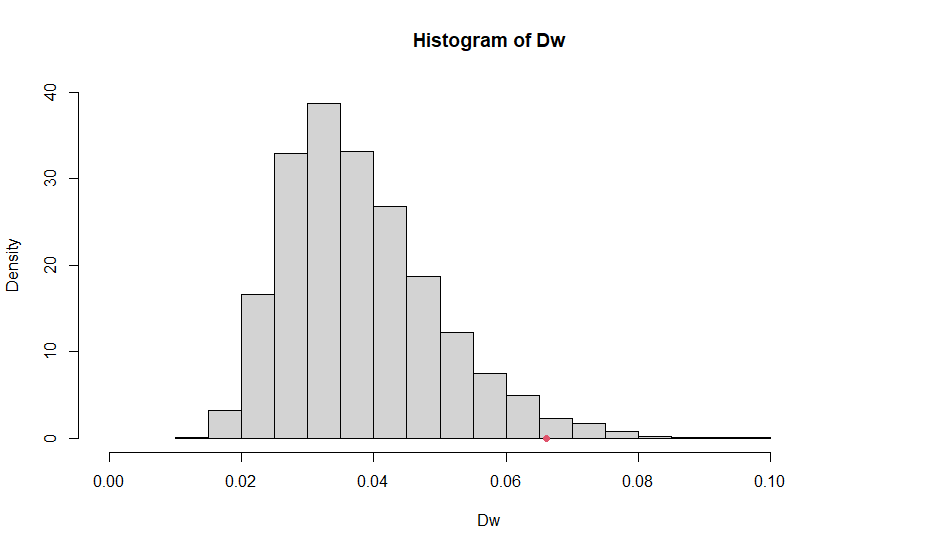
\includegraphics[width=12cm]{Wykresy 11B/11B-MC.png}}

Po przetestowaniu hipotezy zerowej o równości dystrybuant, przy wykorzystaniu metody Monte-Carlo i statystyk Kołmogorowa-Smirnowa, uzyskano wyniki:
  $$ Dw = 0.06613342 $$
  $$p = length(Dw[Dw>dw])/N = 0.0238$$ 

gdzie Dw to odległość dystrybuant empirycznych od rozkładu Weibulla, dw to wartość statystyki Dw, dla danych akcji spółki, N = 10000

\\
Wartość p jest mniejsza od przyjętego poziomu istotności,

   $$ \alpha  = 5\%$$

Zatem hipotezę o równości dystrybuant odrzucamy.





\newpage


\section{Analiza łącznego rozkładu log-zwrotów}
W tym rozdziale wykonujemy analizę dziennych log-zwrotów wcześniej wymienionych spółek: 11 bit studios oraz CD Projekt. 
\begin{figure}[H]
    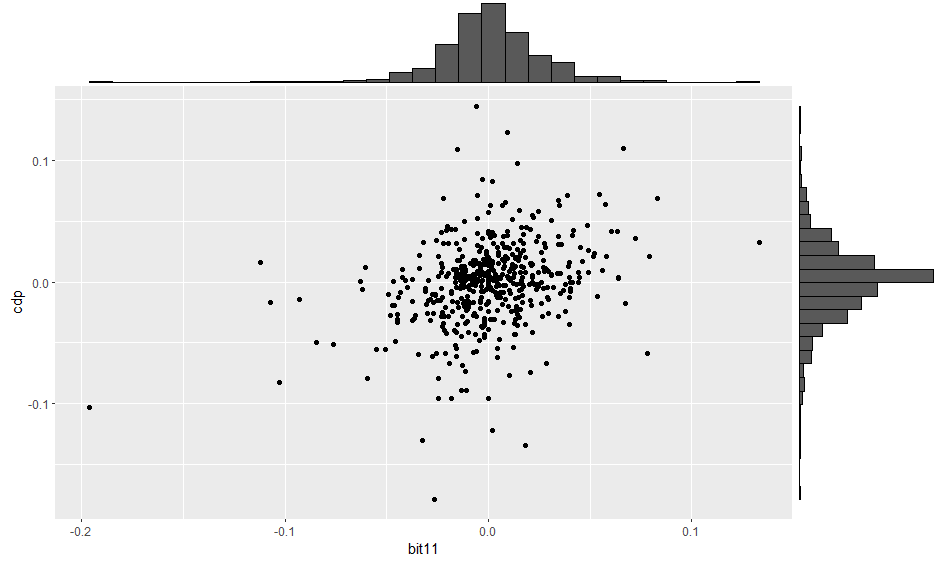
\includegraphics[width=12cm]{Wykresy/Histogram_rozkladow_brzegowych.png}
    \caption{Histogram rozkładów brzegowych}
    \label{Histogram_rozkladow_brzegowych}
\end{figure}
Z powyższego wykresu widać, że dane są znacznie rozproszone. Zauważalna część punktów skupia się wokół wektora średnich. Występuje tu dodatnia zależność. Duża ilość odstających wartości.
\begin{itemize}
  \item Wektor średnich $\hat{\mu}$ = (bit11: 0.000641, cdp: -0.00078)
  \item Kowariancja - cov 0.000311
  \item Współczynnik korelacji - cor 0.32332
\end{itemize} 

Wektor średnich $\hat{\mu}$ świadczy o średniej wartości poszczególnych zmiennych losowych. 

\\
Kowariancja jest bliska 0, oznacza to, że zmienne losowe nie są ze sobą związane w żaden szczególny sposób, istnieje słaby związek pomiędzy zmiennymi losowymi. W takim przypadku zmiany w jednej zmiennej nie są skorelowane z zmianami w drugiej zmiennej, nie występuje żadna zależność liniowa.

\\
Jeśli współczynnik korelacji wynosi 0.32, oznacza to, że istnieje słaba, dodatnia korelacja pomiędzy dwoma zmiennymi losowymi. To znaczy, że wzrost jednej zmiennej wiąże się z wzrostem drugiej zmiennej, ale związek ten nie jest silny. 

Wzór na macierz kowariancji: \\

\centerline{${\Sigma}$ = $\begin{bmatrix}
    Var(X) & cov(X,Y) \\
    cov(Y,X) & Var(Y)
\end{bmatrix}$ = 
$\begin{bmatrix}
    \sigma_1^2 & \rho\sigma_1\sigma_2 \\
    \rho\sigma_1\sigma_2 & \sigma_2^2
\end{bmatrix}$} \\
gdzie $\sigma_1$, $\sigma_2$ to odchylenia standardowe i $\rho$ współczynnik korelacji

\\
Macierz kowariancji dla analizowanych danych: \\
\begin{center}
    $\hat{\Sigma}$ = $\begin{bmatrix}
    0.00077 & 0.00031 \\
    0.00031 & 0.00117
\end{bmatrix}$
\end{center}\\

Wzór na macierz korelacji:  \\
$$\rho =
\begin{bmatrix}
1 & \frac{\text{cov}(X,Y)}{\sigma_X \sigma_Y} \\
\frac{\text{cov}(X,Y)}{\sigma_X \sigma_Y} & 1
\end{bmatrix}$$

\\
Macierz korelacji dla analizowanych danych: \\
\begin{center}
    $\begin{bmatrix}
    1 & 0.32332 \\
    0.32332 & 1
    \end{bmatrix}$
\end{center}


\begin{figure}[H]
    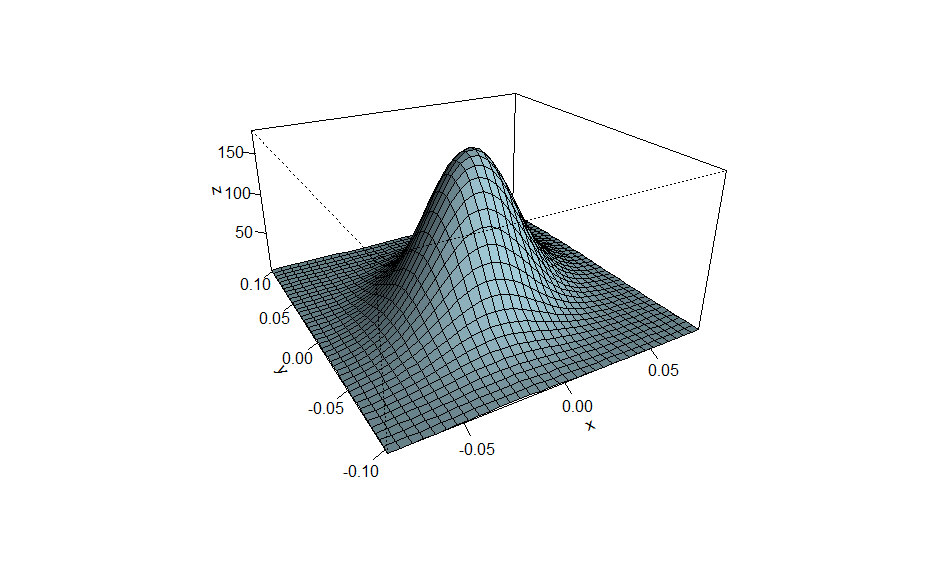
\includegraphics[width=12cm]{Wykresy/Wykres_gestosci.png}
    \caption{Wykres gęstości}
    \label{Wykres_gestosci}
\end{figure}

\newpage

Gęstość rozkładu normalnego o wyestymowanych parametrach  jest zapisywana w następujący sposób:


$$f(x, y) = \frac{1}{2\pi\sigma_1\sigma_2\sqrt{1 - \rho^2}} \exp\left(-\frac{1}{2(1 - \rho^2)}\left[\frac{(x - \mu_1)^2}{\sigma_1^2} - 2\rho\frac{(x - \mu_1)(y - \mu_2)}{\sigma_1\sigma_2} + \frac{(y - \mu_2)^2}{\sigma_2^2}\right]\right)$$

gdzie $x$ i $y$ są wektorami zmiennych losowych, $\hat{\mu}$ jest wektorem średnich, $\sigma_1$, $\sigma_2$ to odchylenia standardowe i $\rho$ współczynnik korelacji.\\
\\
Gęstość rozkładu normalnego dla analizowanych danych:

$$f(x, y) = 177.23\cdot\exp(-725.15(x-0.00064)^2 + 380.07(x-0.00064)(y+0.00078)$$
$$-477.24(y + 0.00078)^2)$$


\\
Gęstość rozkładów brzegowych jest zapisywana w następujący sposób:


$$f(x) = \frac{1}{\sigma\sqrt{2\pi}}\exp\left(-\frac{(x-\mu)^2}{2\sigma^2}\right)$$

\\

Gęstość rozkładów brzegowych dla analizowanych danych:


$$f_{11b}(x) = 14.39388\cdot\exp\left(-\frac{(x-0.00064)^2}{0.00154}\right)$$


$$f_{cdr}(x) = 11.65201\cdot\exp\left(-\frac{(x+0.00078)^2}{0.00234}\right)$$


\begin{figure}[H]
    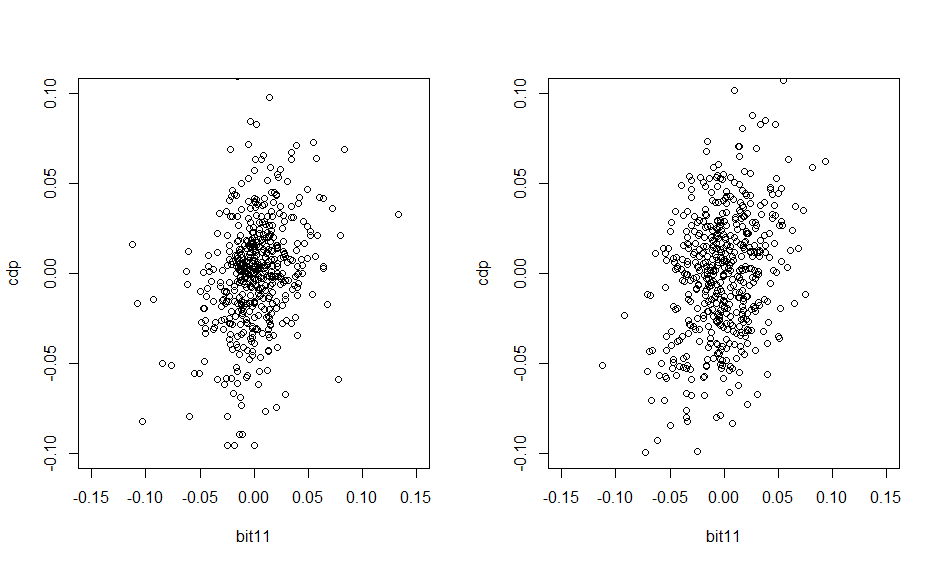
\includegraphics[width=12cm]{Wykresy/QQploty.png}
    \caption{Wykresy rozrzutów: pierwszy -otrzymany na podstawie danych, drugi - w oparciu o wygenerowaną próbę}
    \label{QQploty}
\end{figure}
Po wygenerowaniu próbę liczności danych = 509, na powyższym wykresie widać, że nasze dane nie przypominają rozkładu normalnego. Skupienie danych na obu rozkładach jest różne. Jest też wiele wartości odstających.
\\ \\
\newpage
Badanie hipotezy mówiącej o tym, że kwadrat odległości Mahalanobisa wektora cen od średniej ma rozkład $\chi^2$ (drugiego stopnia).
\begin{figure}[H]
    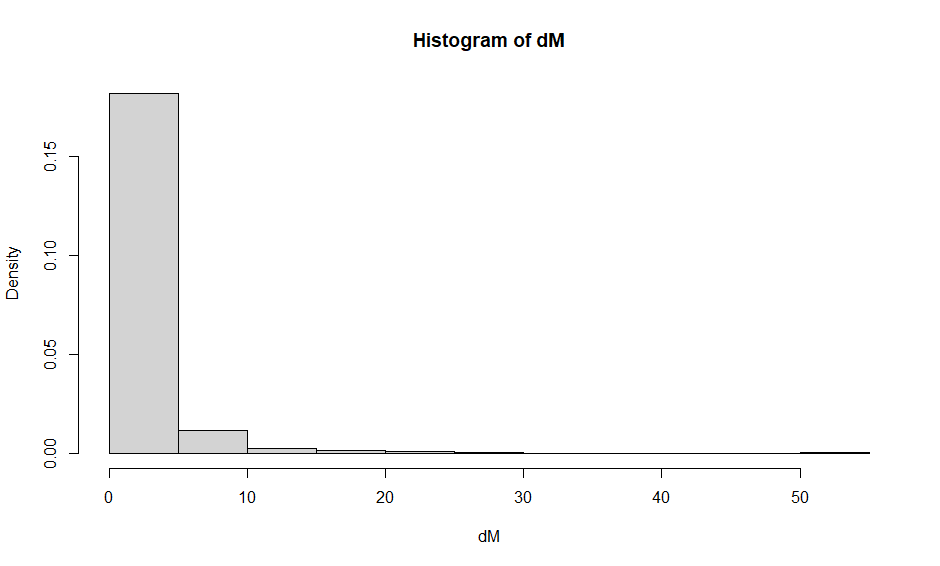
\includegraphics[width=12cm]{Wykresy/Histogram_Mahalanobis.png}
    \caption{Histogram kwadratów odległości Mahalanobisa}
    \label{Histogram_Mahalanobis}
\end{figure}
Zasadnicza większość wartości znajduje się w pierwszym przedziale. Histogram nie ma zbliżonego kształtu do rozkładu $\chi^2$ (drugiego stopnia) -  ma dużą wartość na początku, a następnie bardzo małe, wręcz bliskie zeru (nie jest tak "płynny" jak powinien być).
\\
\\
Po przeprowadzeniu analizy statystycznej rozkładów kursów ustaliliśmy, iż najbardziej odpowiedni model dla opisania tych danych jest rozkład normalny dwuwymiarowy. W konsekwencji, kwadrat odległości Mahalanobisa od średniej powinien być rozłożony według rozkładu$\chi^2$(2).

\begin{figure}[H]
    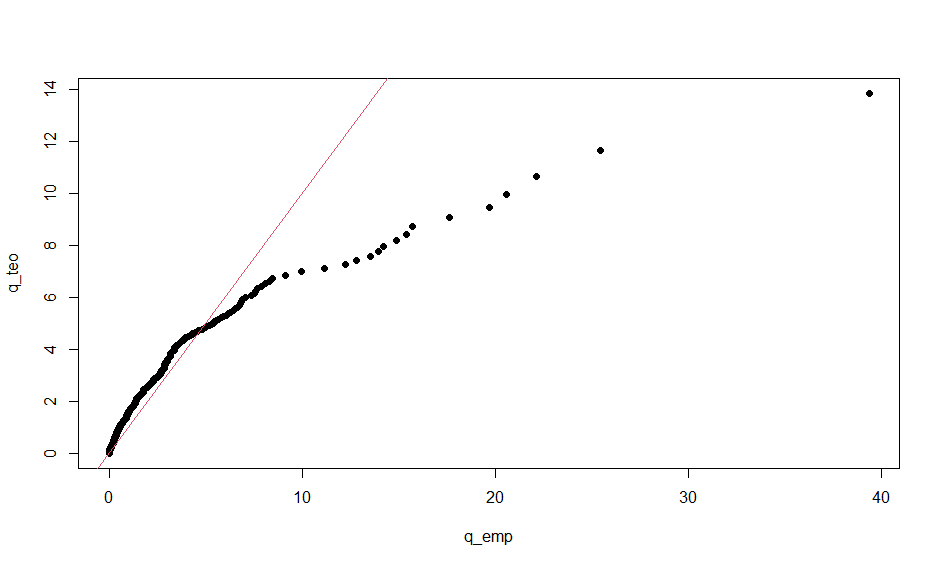
\includegraphics[width=12cm]{Wykresy/QQplot_Mahalanobis.png}
    \caption{Wykres diagnostyczny typu QQ-plot}
    \label{QQplot_Mahalanobis}
\end{figure}
 Analiza Q-Q plot wykazała, że rozkład $\chi^2$ (stopnia drugiego) nie jest odpowiedni do opisu naszych danych empirycznych. Porównanie danych teoretycznych (przedstawionych przez czerwoną linię) z danymi empirycznymi (przedstawionymi przez czarne punkty) wykazało istotne odchylenia, co sugeruje potrzebę poszukiwania innego rozkładu statystycznego dla opisu tych danych.

\\

Za pomocą testu zgodności badamy czy dane empiryczne pochodzą z rozkładu $\chi^2$ (stopnia drugiego). Celem testu jest zweryfikowanie hipotezy zerowej, oraz hipotezy alternatywnej, która głosi, że dane nie pochodzą z tego rozkładu. W teście uzyskamy wartość p, które pozwali na ocenę poziomu istotności statystycznej odchyleń danych od rozkładu teoretycznego.

\newpage


Po przetestowaniu hipotezy że kwadrat odległości Mahalanobisa wektora cen od średniej mają rozkład $\chi^2$ (stopnia drugiego), przy wykorzystaniu metody Monte-Carlo i statystyk Kołmogorowa-Smirnowa, uzyskano wyniki:
  $$ D = 0.16836 $$
  $$ p = 5.882e^{-13} $$ 

Wartość p jest mniejsza od przyjętego poziomu istotności:

   $$ \alpha  = 5\%$$
   
Oznacza to, że jest bardzo mało prawdopodobne, że dane empiryczne pochodzą z rozkładu $\chi^2$ (stopnia drugiego). Wartość p jest mniejsza niż poziom istotności $ \alpha  = 5\%$, zatem odrzucamy hipotezę zerową i przyjmujemy hipotezę alternatywną. Ponadto, przez to odrzucamy również hipotezę o normalności rozkładu log-zwrotów dla badanych spółek.


\section{Regresja liniowa dla log-zwrotów}


\textbf{Przedziały ufności dla wartości oczekiwanych log-zwrotów spółki CDR.}
\\
\\
Wykorzystywany jest Model 2, z uwagi na dużą ilość próbki oraz na brak jej normalności.

Wzór dla przedziału ufności dla Modelu 2 będzie następujący:

$$[\overline{X}_n - \mu(1-\alpha/2)\cdot\frac{S_n}{\sqrt{n}}, \overline{X}_n + \mu(1-\alpha/2)\cdot\frac{S_n}{\sqrt{n}}]$$

gdzie; $\mu$ = -0.0007792008, $S_n$ = 0.03423808, $X_n$ = log-zwroty spółki, dla danych długości n = 509 i $\alpha$ =  5\%
\begin{itemize}
 \item przedział lewy wynosi: -0.003753595
\item przedział prawy wynosi: 0.002195194
\end{itemize} 
Ostateczny przedział ufności dla wartości oczekiwanych log-zwrotów spółki CDR wynosi:
[-0.003753595, 0.002195194]

\newpage
\\
\textbf{Przedziały ufności dla wartości oczekiwanych log-zwrotów spółki 11B.}

\\
\\
Wykorzystywany jest Model 2, z uwagi na dużą ilość próbki oraz na brak jej normalności.
\\
Wzór dla przedziału ufności dla Modelu 2 będzie następujący:

$$[\overline{X}_n - \mu(1-\alpha/2)\cdot\frac{S_n}{\sqrt{n}}, \overline{X}_n + \mu(1-\alpha/2)\cdot\frac{S_n}{\sqrt{n}}]$$

gdzie; $\mu$ = 0.0006374281, $S_n$ = 0.02771611, $X_n$ = log-zwroty spółki, dla danych długości n = 509 i $\alpha$ =  5\%
\begin{itemize}
 \item przedział lewy wynosi: -0.001770378
\item przedział prawy wynosi: 0.003045234
\end{itemize} 
Ostateczny przedział ufności dla wartości oczekiwanych log-zwrotów spółki 11B wynosi:
[-0.001770378, 0.003045234]
\\
\\
\textbf{Estymatory:}
$$\beta_1\ = \frac{cov(X,Y)}{\sigma_x^2} = 0.2617344 $$ 
$$\beta_0\ = \overline{X} -\overline{Y} * \beta_1\ =  -0.0009460377 $$ 
gdzie X to log-zwroty dla spółki CDP, a Y dla spółki 11B
\\
Nasz model to $$ y = \beta_0 + \beta_1 \cdot x = -0.0009460377 + 0.2617344 \cdot x $$

\newpage
\textbf{Analiza Regresji}

\begin{figure}[H]
    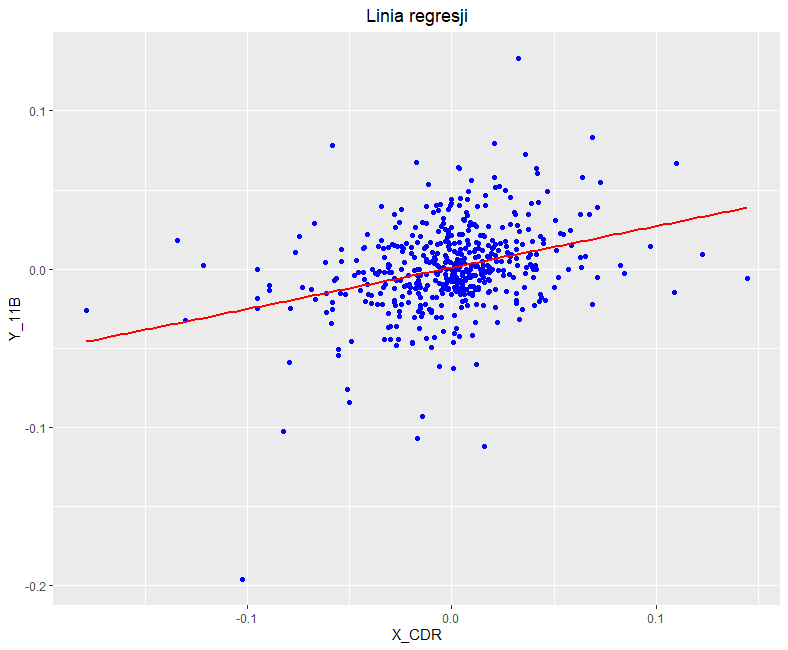
\includegraphics[width=12cm]{Wykresy/Prosta regresji.png}
    \caption{Linia regresji na  wykresie}
    \label{Wykres_regresji}
\end{figure}


\begin{figure}[H]
    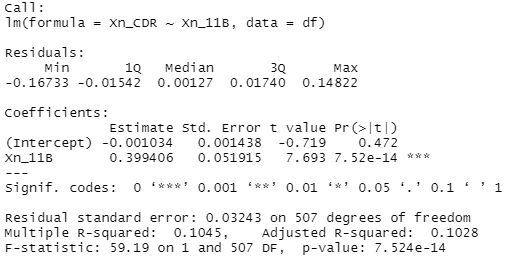
\includegraphics[width=11cm]{Wykresy/Analiza.png}
\end{figure}

\\
Powyższy wynik pochodzi z analizy regresji liniowej, gdzie zmienna zależna ($Y_{11B}$) jest przewidywana przez zmienną niezależną ($X_{CDR}$) i jest to przedstawiane za pomocą prostej na wykresie. 
\\\\
Tabela "Coefficients" pokazuje oszacowane współczynniki dla przecięcia i zmiennej niezależnej. Wartość $t$ dla zmiennej niezależnej wynosi 7.693, a wartość $p$ i $F-statistic$ wynoszą kolejno: $7.52e^{-14}$ i 59.19, co sugeruje, że zmienna niezależna jest istotnym czynnikiem wpływającym na zmienną zależną.
\\
\\
W przedstawionych danych widzimy, że reszty mają wartości minimalne -0.170289, maksymalne 0.123715 i kwartyle: 1Q -0.012718, Mediana -0.000841, 3Q 0.014242. Z tego możemy wywnioskować, że reszty są dość małe i rozłożone wokół zera, co jest zgodne z założeniem, że reszty powinny być rozłożone normalnie o średniej 0 i stałym rozkładzie. 
\\\\
Średni błąd ($\sigma^2$)  jest równy 0.02625, ma on małą wartość co świadczy o dobrym dopasowaniu modelu. 
Stopnie swobody oznaczają liczbę niezależnych punktów danych, które służą do estymacji parametrów modelu. W tym przypadku jest to 507, co sugeruje, że model jest dobrze dopasowany do danych i ma wysoką precyzję.
\\
\\
R-kwadrat (współczynnik determinacji) to stosunek wariancji składników modelu do wariancji danych. Wynosi on 0.1028, co oznacza, że zmienna niezależna wyjaśnia około 10\% wariancji zmiennej zależnej. Zatem 90\% zmienności  nie jest wyjaśniona przez obecne zmienne. Można więc rozważyć dołączenie do naszego
modelu jeszcze innych zmiennych.
\\\
\\
\textbf{Test istotności współczynników $\beta_0$, $\beta_1$.}
\\

Sprawdzamy hipotezę zerową $\beta_0=0$, przeciwko alternatywnej hipotezie $\beta_0\neq0$ oraz sprawdzamy hipotezę zerową $\beta_1=0$, przeciwko alternatywnej hipotezie $\beta_1\neq0$.
\\\\
Dla współczynników $\beta_0$ i $\beta_1$ odchylenia estymatorów wynoszą:
\begin{itemize}
\item $\beta_0$ = 0.001163958
\item $\beta_1$ = 0.03402064
\end{itemize} 
\\
Wartości $t_0$ i $t_1$ to wartości statystyki T, które służą do testowania hipotezy zerowej o braku istotności współczynników regresji. wynoszą odpowiednio:
\begin{itemize}
\item $t_0$ = -0.8127763
\item $t_1$ = 7.693402
\end{itemize} 

\newpage
 Wartość $p-value$ ($p$ = P(|T|>t0), $p$ = P(|T|>t1)) to prawdopodobieństwo, że wartość statystyki T jest większa niż wartość obliczona dla danych.

\begin{itemize}
\item $p-value$ = ($p$ = P(|T|>t0), $p$ = P(|T|>t1))
\item $p-value$ dla $t_0$ =  0.4183785
\item $p-value$ dla $t_1$ = $1.325384^{-11}$
\end{itemize} 


 Wartość $p-value$ dla współczynnika $\beta_0$ jest równa 0.4183785, co oznacza, że można przyjąć hipotezę zerową $\beta_0=0$ i pominąć $\beta_0$ z modelu. Wartość $p-value$ dla współczynnika $\beta_1$ jest równa $1.325384^{-11}$, co oznacza, że nie ma podstaw do odrzucenia hipotezy zerowej, że współczynnik $\beta_1$ jest równy zero.
 \\\\
\textbf{Analiza reszt}
\\
Testujemy hipotezę czy dystrybuanta reszt ma rozkład normalny o średniej i wariancji z próby, oraz kontr hipotezę, że nie ma ona rozkładu normalnego.

 \begin{figure}[H]
    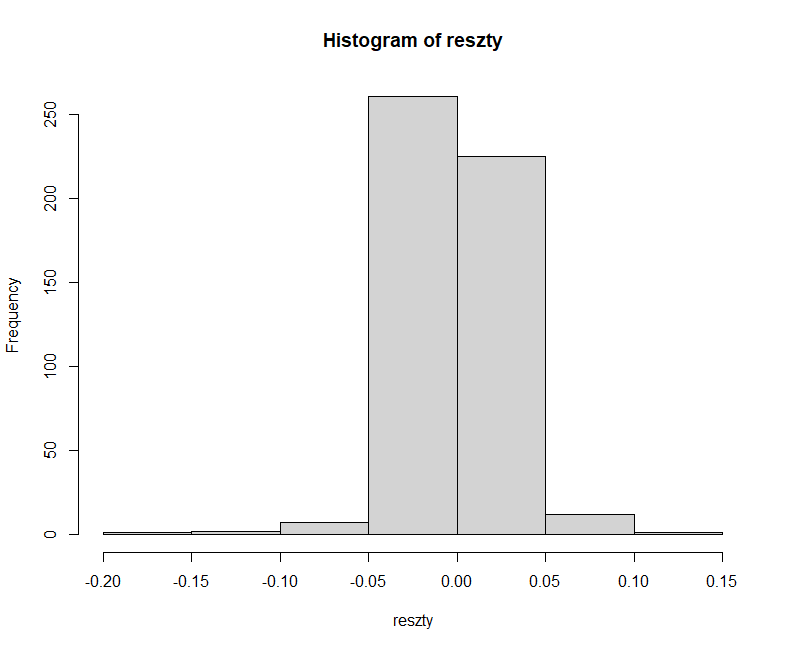
\includegraphics[width=12cm]{Wykresy/histogram reszty.png}
    \caption{Na histogramie widać, że większość reszt wpada w przedziały od -0.05 do 0.05 i wpisuje on się w kształt rozkładu normalnego}
\end{figure}

 \begin{figure}[H]
    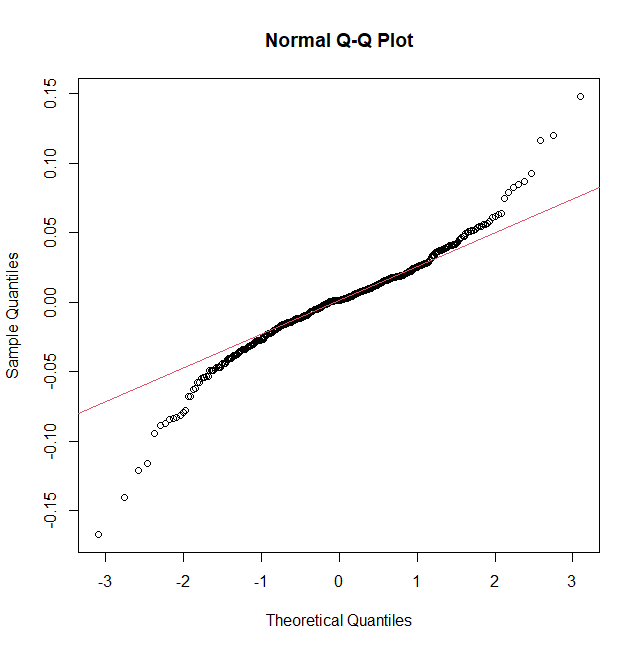
\includegraphics[width=12cm]{Wykresy/qqplot reszty.png}
     \caption{Na wykresie kwantyl-kwantyl widać iż znaczna cześć empirycznych pokrywa się z linią która reprezentuje dane teoretyczne, co sugeruje że reszta będzie z rozkładu normalnego}
     
\end{figure}

\begin{itemize}
\item Średnia reszt = $6.525989^{-19}$
\item odchylenie = 0.02622743
\end{itemize} 

Średnia reszt jest bliska zeru, co oznacza, że w średnim model przewiduje dobrze wartości zmienności $R^2$. Natomiast odchylenie standardowe reszt wynosi 0.02622743, co oznacza, że większość reszt znajduje się w przedziale od -0.02622743 do 0.02622743 od wartości przewidywanej.
\\\\
Z pomocą testu Kołmogorowa-Smirnova sprawdzamy czy dane należą do rozkładu normalnego.
Uzyskane wyniki:
\\
\begin{itemize}
\item D = 0.081221
\item $p-value = 0.002424$
\end{itemize} 

 $p-value$ jest mniejsze niż 0.05, co sugeruje, że nie ma podstaw, by odrzucić hipotezę, że reszty są normalnie rozłożone.

$$ RSE = 0.02624$$

 Błąd standardowy reszty RSE jest miarą, jak dobrze model matematyczny opisuje dane. Oznacza on średni odchylenie reszt (różnica między wartością rzeczywistą a przewidywaną przez model) od wartości średniej. Im mniejszy błąd standardowy reszty, tym lepiej model opisuje dane. Wartość 0.02624 wskazuje, że nasz model jest precyzyjny.

\\\\
Na podstawie powyższych analiz można uprościć model o pominięcie $\beta_0$,
Po dokonaniu ponownej regresji model prezentuje się tak: 
$$model.lm2 = lm(Y_{11B} \char`\~ X_{CDR}-1,data=df)$$ 
$$ y = \beta_1*x$$
a jego podsumowanie tak:
 \begin{figure}[H]
    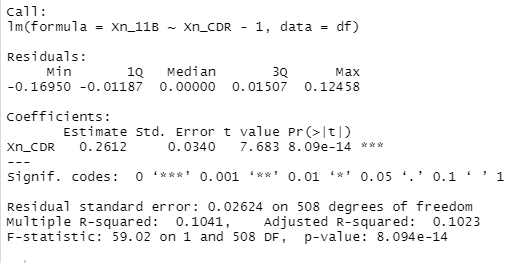
\includegraphics[width=12cm]{Wykresy/model_nowy.png}
    \caption{Nowy model po pominięciu b0}
\end{figure}
\\
 Nowy model jest minimalnie lepszy, ponieważ ma więcej stopni swobody (508 w porównaniu z 507 w pierwszym modelu).

\\\\
 \textbf{Wielkości log-zwrotów spółki 11B, gdy log-zwroty spółki CDR będą na poziomie średniej z posiadanej próby.}

predykcja będzie następująca:

$$\beta_{1 model2}*m =-0.0002035073  $$
$$m_{CDR}= -0.0007792008 $$

Przedziały ufności:
\begin{table}[H]
\centering 
\begin{tabular}{|l|l|l|l|l|}
\hline
fit & lwr & upr \\ \hline
-0.0002035073 & -0.0002555499 & -0.0001514647 \\ \hline
\end{tabular}
\end{table}

Przedział ufności jest to zakres, w którym znajduje się prawdziwa wartość zmiennej, z pewnym poziomem pewności. Wartość "fit" jest oszacowaną wartością, a "lwr" i "upr" są dolnym i górnym ograniczeniem przedziału ufności, odpowiednio. W tym przypadku mówimy, że z pewnym poziomem ufności, prawdziwa wartość zmiennej znajduje się pomiędzy "lwr" a "upr". 

\section{Podsumowanie}
Celem projektu była analiza spółek CDR i 11B, którą podzieliśmy na 3 etapy.
\\

Pierwszy etap skupiał się na cenach zamknięcia akcji spółek, przedstawialiśmy wykresy kursów, szukaliśmy rozkładu który by jak najlepiej opisywał powyższe dane, za pomocą wartości statystyk, kryteriów informacyjnych i metody Monte-Carlo. Niestety, dla żadnej ze spółek dobrane rozkłady nie były wystarczająco pasujące. 
\\

Drugi etap obejmował analizę dziennych log-zwrotów spółek. Dokonaliśmy analizy dopasowania rozkładu normalnego do danych, przy użyciu m.in kwadratów odległości Mahalanobisa. Badanie zakończyło się odrzuceniem hipotezy o normalności rozkładu. 
\\

W trzeciej części zajęliśmy się tworzeniem modelu regresji liniowej. Po przeanalizowaniu parametrów model udało się uprościć. Następnie wyliczyliśmy predykcję dla wielkości log-zwrotów spółki 11B, gdy log-zwroty spółki CDR będą na poziomie średniej z posiadanej próby.
\\

Ostatecznie, nasze wyniki sugerują konieczność bardziej zaawansowanego podejścia do analizy cen, aby lepiej zrozumieć rynkowe trendy i przewidzieć możliwe scenariusze.
\end{document}

\\ \hline